\documentclass[midd]{thesis}

\usepackage{tikz}
\usetikzlibrary{matrix,chains,positioning,decorations.pathreplacing,arrows}

\usepackage{graphicx}
\usepackage{times}
\usepackage{longtable}
\usepackage{ctable}

\bibliographystyle{plain}

\title {Combating Fraud By Leveraging Machine Learning and Human Behavior}

\author {Casey Astiz}
\adviser {Professor Michael Linderman}

\begin{document}

\maketitle
\pagenumbering{roman}

\begin{abstract}
I am writing about fraud and how to detect it! Wooh!
\end{abstract}

\begin{acknowledgements}
I would like to thank Professor Linderman and Professor Scharstein first and foremost for their help in this Computer Science Thesis. Without them, this thesis would cease to exist. I would also like to thank the Computer Science department at Middlebury College for giving me the opportunity to learn and develop as a computer scientist. Last, I would like to thank all my unnamed interviewees who were willing to discuss their expertise about fraud detection with me. I truly appreciate all who helped create this thesis, and add to my knowledge!

\end{acknowledgements}

\contentspage
\tablelistpage   
\figurelistpage

\normalspacing \setcounter{page}{1} \pagenumbering{arabic}

\chapter{Introduction}
\label{sec:intro}


Every day there are new ways to pay for goods or services. As shown in Figure ~\ref{fig:paymentMethods}, cash is a way of the past; mobile, peer to peer, and online payments through credit cards are the way of the future \cite{paymentMethods}. While these convenient payment methods are very exciting, the additional methods of payment lead to increased opportunities for fraud. Credit card fraud is on the rise, with the United States reaching \$8 billion in 2018 as seen in ~\ref{fig:USA}  \cite{USA}. High valued fraud is happening all over the world, and it is necessary to find more efficient and effective methods to catch fraudsters to keep everyday users safe unaffected by fraud. For example, credit card fraud through online payments in Australia hit \$476 million in 2017, rising \$58 million from the year before \cite{Wang2018}. 

Financial fraud increases costs to a company through several means. With any type of financial fraud, there is a certain level of financial burden for the company or bank that has to pay out. Other than the cost of the fraudulent transaction itself, having high levels of fraud leads to uncertainty for both the customers and bank trustees. This uncertainty then creates higher transaction costs for all and less efficient markets. When banks lose money to fraudsters, card holders partially or entirely pay for this loss through higher interest rates, fees, or reduced rewards and benefits for customers. Without automatic fraud detection, a significant amount of overhead exists because of the cost of investigating transactions and employing these investigators \cite{Chan}. However, credit card fraud is not only important for the bottom line, as ``credit card frauds have important social consequences and ramifications, as they support organized crime, terrorism funding, and international narcotics trafficking" \cite{Zanin2018}.

\begin{figure}
  \includegraphics[scale=0.5]{paymentMethods.png}
  \caption{Leading payment methods in the United States in 2017 \cite{paymentMethods}}
  \label{fig:paymentMethods}
\end{figure}

Fraud detection is an instance of anomaly detection. Fraud detection and anomaly detection more broadly are difficult problems because of the heavily skewed classes and potential for intermingled classes. These two features means that there are few examples for classifiers to learn, and there may not be a clear line to divide classes by. Further, an effective fraud detector must be adaptive to new patterns and categories of fraud. The main goal of this thesis is to investigate current methods of financial fraud detection and implement one or more of those methods. I will describe the most prevalent methods for fraud detection in current use, as well as past fraud detection methods.

Chapter~\ref{sec:background} reviews different methods used in the industry in the past and present for fraud detection. The background section will combine information from research papers with Chapter~\ref{sec:context}, which synthesizes information I learned from interviewing people at different companies in this field to provide some context for the literature review. My own implementation of a fraud detection system is described in Chapter~\ref{sec:impl} using a synthetic credit card transaction dataset. Comparing business interactions with fraud to published research in the field will allow me to somewhat analyze the performance of different fraud detection methods in real life versus a research context. Chapter~\ref{sec:future} will discuss other applications for successful fraud detectors. Chapter ~\ref{sec:conclusion} concludes.

\begin{figure}
  \includegraphics[scale=.5]{USA.png}
  \caption{Value of payment card fraud losses in the United States from 2012 to 2018, by type (in billion U.S. dollars) \cite{USA}}
  \label{fig:USA}
\end{figure}


\pagebreak

\chapter{Fraud Detection}
\label{sec:background}

Here we define fraud as ``wrongful deception with the intent to gain personally or financially," or intentionally deceiving another person to obtain their property \cite{legaldict}. Fraud can either be a civil or criminal offense, depending on the state. There are a multitude of types of frauds, from credit card fraud and website misdirection to pyramid schemes and insurance fraud. It is important for businesses to balance finding all fraud and limiting their customers. A company may choose to accept some level of fraudsters in order to maximize the amount of legitimate users being classified as fraudsters. For example, in subscription based services, it can be less expensive for companies to accept all potential users to create new accounts because the cost of losing a potential client can be higher than the cost of allowing a small portion of fraudulent accounts. Because companies are normally profit maximizing, fraud detection in a business context will most likely always involve weighing the costs of false positives.

Researchers have more flexibility than a financial institution in their pursuit of fraud detection. Researchers are able to manipulate datasets by artificially changing fraud versus non-fraud proportions, and testing different combinations for the best performance. Researchers also have no time restraints as they do not need to make a split second decision of whether or not to allow or deny a transaction. Some may look for performance gains for in the moment decision making, but researchers can build systems that make decisions in any amount of time. The lack of restraints allows for a breadth of study into potential solutions to fraud detection. 

\section{Imbalanced Classes} %% fix combo of stolfo papers

Financial fraud detection falls under the category of anomaly detection because of the heavily skewed classes. Some datasets are perfectly split between two classes. This means that there are equal amounts of positive and negative examples for a classifier to be trained with. Imbalanced classes happen when there is more examples of one class over another, and is commonly used to refer to large differences in amount of examples. This imbalance makes classifying the minority class more difficult because the classifier has not seen as many examples of that class, and therefore the model's weights will be biased towards the majority class. Anomaly detection is an extreme example of skewed classes because the minority could be less than 1\% of the examples. Therefore, it is likely a system will default to predicting only the majority class and still have high accuracy.

There are a few ways to model skewed data with classifiers. One basic and effective strategy is to get more data. With more examples of the anomaly, it is easier to detect a pattern between them. However, acquiring more data is not always an option, especially when working with data collected in the real world. Another popular method for dealing with data imbalance is to artificially balance the data.  In a study by Chan and Stolfo from 1998, the authors find that artificially balancing the data leads to more accurate classifiers \cite{Chan}. To balance the classes, one can under sample the majority class or over sample the minority class by creating more instances of minorities.


Chan and Stolfo also implement a cost-sensitive approach to measure the success of their classifiers. In most machine learning problems, the default metric to monitor a model is accuracy of a system. However, this is not an effective measure when discussing anomalies. For example, in my own implementation, if a classifier were to predict non-fraud for each transaction, the accuracy would be over 99\%, but would still not be catching any of the fraud. Metrics that are often used to measure skewed class problems are precision, recall, and F1 score. These all combine ratios of true positives to false positives, analyzing the success in predicting the minority class rather than the majority class. Chan and Stolfo take a new approach, and instead use the average aggregate cost of fraud as their metric for evaluating their model \cite{Chan}. In addition to tracing the performance with different data distributions, the authors also look at costs including different levels of overhead costs.  

Figure~\ref{fig:chan} shows the results of Chan and Stolfo's system. While they find that larger overhead leads to higher overall cost, they also notice that when overhead is smaller, cost is minimized at a larger percentage of fraudulent transactions in the training set. When overhead is smaller, a bank can afford to have a higher false positive rate, as the false positives can be investigated relatively inexpensively. When overhead is larger, a bank cannot afford as many false positives, as it is expensive to investigate all of the false positives, but would rather have a higher false negative rate. These results are helpful for banks who may be deciding where to focus their resources.


\begin{figure}
  \includegraphics[scale=0.5]{chan_stolfo.png}
  \caption{Training Distribution vs. the credit card fraud cost model \cite{Chan}}
  \label{fig:chan}
\end{figure}

%To address skewed classes, Chan and Stolfo implement a cost-sensitive approach instead of using an accuracy based error rate. Because of the skewed class, accuracy is a poor measure for system performance; a system that only predicts non-fraud will still have a high accuracy. Instead, they analyze their models using the value of the fraud as their metric. They use a multi-classifier meta-learning approach, where they create data subsets with appropriate class distributions and apply learning algorithms to subsets called local fraud detection agents. The collective knowledge learned from the local fraud detection agents is then combined using meta learning. The benefit of this approach is that it handles non-uniform cost per error and is cost sensitive during the learning process. Chan and Stolfo use a dataset from Chase Manhattan Bank containing half a million transactions, from which 20 \% are fraudulent, and implemented a cost model based on information from a bank representative. This is a relatively high percentage of fraud, as fraud today makes up closer to 1-3\% of transactions.
%
%Given this data and information, the authors experimented with the effects of training class distributions on the credit card cost model. They used the first 10 months as training data and the 12th month for testing, and randomly sampled transactions to get varied fraud amounts. The multi-classifier meta learning approach works by randomly dividing the dataset into 4 subsets, and then learns on the subsets using one of four algorithms: CART, C4.5, RIPPER, or BAYES. The authors found that the training class distribution can affect the performance of the learned classifier, which is an issue given that financial transactions can have any class distribution. However, this research shows that artificially changing these data proportions is effective. Additionally, they found their method to be efficient and scalable for large datasets as well as flexible. This modular multi-classifier approach facilitates adaptive learning over time in the local agents and removal of out-of-date learned behavior.

A 1997 paper by Stolfo et al uses Meta-Learning for credit card fraud detection \cite{Stolfo1997}. Here, the authors similarly argue that a false positive rates and true positive rates are much better metrics than overall accuracy when evaluating these learned fraud classifiers. Their proposed meta-learning system allows financial institutions to share their models of fraudulent transactions by exchanging classifier agents in a secured agent infrastructure. This is a useful tool for financial institutions to be able to work together to solve similar fraud problems. 

%% Meta-learning is a general strategy that provides a means for combining and integrating a number of separately learned classifi- ers or models. A meta-learning system allows financial institutions to share their models of fraudulent transactions by exchanging classifier agents. -- from a different paper

For this study, the authors used a database of 500,000 transaction records from the Financial Services Technology Consortium, each containing 30 fields. In their experiment, the authors tested various machine learning and meta-learning models with different proportions of fraud to non-fraud training data. Based on their experiments, they find that a 50\%/50\% distribution of fraud to non-fraud training data generates classifiers with the highest true positive rate (80\%) and the lowest false positive rate (13\%). The best method the authors discovered is using meta-learning with BAYES as a ``meta-learner to combine base classifiers" \cite{Stolfo1997}. For reference, BAYES is very similar to logistic regression, as it takes features as input and outputs a probability.

\section{Credit Card Fraud}

The papers in the previous section mainly focus on redistributing the imbalanced classes as a way to improve fraud detection rates. Zanin et al take a new approach to credit card fraud detection. Here, the authors use parenclitic network analysis, which is a hybrid data mining and complex network classification algorithm \cite{Zanin2018}. In general, a parenclitic network is a network reconstruction technique that allows highlighting of the differences between one instance and a set of standard instances. These parenclitic networks are summaries of the groups of features whose correlation differs from a normal or licit transaction. Therefore, the structure of a parenclitic network stores information about abnormal correlated features in a credit card transaction. An example of parenclitic network creation is shown in Figure~\ref{fig:parenclitic}. 

\begin{figure}
\centering
  \includegraphics[scale=0.5]{parenclitic.jpg}
  \caption{Parenclitic Network Formation \cite{Boccaletti}}
  \label{fig:parenclitic}
\end{figure}

The authors take the computed network and transform it into a set of features compatible with a data mining algorithm like a multi-layer perceptron.  The authors argue that fraud detection is a similar problem to designing a recommendation machine or diagnostic medical tools, which suggests a complex network approach may be beneficial.  Zanin et al combine data mining techniques to extract additional features from the data with a networking approach, which adds the ability to synthesize metrics to describe a ``global structure created by the interactions between the different features" \cite{Zanin2018}. Succinctly, the data mining creates new features, and the network finds connections between these features.  This study uses parenclitic networks, and evaluates them on a dataset of real transactions in comparison to the results of a ANN approach. 

\begin{figure}
\centering
  \includegraphics[scale=0.5]{parenclitic2.png}
  \caption{Overall system \cite{Zanin2018}}
  \label{fig:parenclitic2}
\end{figure}

To test their parenclitic network approach, the authors used an anonymized dataset of all credit and debit card transactions from clients of a Spanish Bank, BBVA, from January 2011 to December 2012. This dataset includes standard fields about transactions such as amount, origin and destination. The authors have also synthesized information like average transaction size for a user from the given information. They use multi-layer perceptrons, a type of ANN, as the model for classifying their transactions. These multi-layer perceptrons are represented by a set of connected nodes in which each connection has a weight associated with it that can be adjusted. The overall system that the authors create is displayed in Figure~\ref{fig:parenclitic2}. Zanin et al find that parenclitic networks alone are not enough to significantly lower the classification error. However, the addition of parenclitic features to the raw data set increases the overall information a model receives as input, decreasing the error rate from 19.2\% to 12.23\% \cite{Zanin2018}. 

In a 2017 paper, Wedge et al have attempted to solve the ``false positive" problem in fraud prediction at an industrial scale \cite{Wedge}. The goal of this paper is to use a feature engineering approach to reduce false positives. It is estimated that only 1 in 5 transactions that are predicted to be fraud are actually fraud, and analysts have found that these false positives are costing more than the fraud itself \cite{Wedge}. However, improving false positive rates with human involvement is very costly, prompting Wedge et al to study the automatic method by the name of deep feature synthesis. The dataset the authors use contains roughly 9.5 million transactions with approximately 112,000 fraudulent transactions. 

The authors create their features using only transaction information and aggregated historical information. These transactions were classified using scikit-learn's random tree classifier with 100 trees. Decision trees are effective at calculating relative feature importances. In addition to this random forest, the authors use a deep feature synthesis algorithm to automatically derive behavioral features based on historical data of the card. This is achieved by looking for relationships between transaction entities, which are transaction groups with multiple transactions and features to describe each transaction. Through these methods, they were able to reduce false positives by 54\% compared to the current BBVA solution \cite{Wedge}. 

They found that their solution can maintain similar benefits when the historical features of a card are computed once every 7 days. This eliminates the need for streaming computing in regards to the feature set because the features can be computed after a period of time instead of constantly updating the feature space. The author's system reduced the false positive rate, and reached an F score of 0.56 versus the BBVA system of 0.20. In addition, Wedge et al's system still reduced total cost to this bank by 190,000 euros. This research is helpful because it shows that features do not need to be recomputed with each new transaction, and that banks can reduce their false positives without increasing the latency for their users.

Both Zanin et al and Wedge et al have successful results, but demonstrate potential problems if fraud detection. Researchers are in a world without time constraints. Therefore, if a classifier takes long periods of time to train, it is not a major concern. However, if the lessons learned from research are to be applied to real world systems, it may be necessary to check potential latency gains for a user. For example, Zanin et al are looking to create more features that help capture what makes a transaction out of the norm. While these parenclitic networks were creating specific and meaningful features, they needed to be combined with features from the initial data. This means that the problem is getting more complicated and computationally expensive, adding time to training. Similarly, Wedge et al are working with a large feature space because of the dataset they were given. This draws attention to the need to preprocess data to ensure time is not being wasted on features that do not benefit the model. Without specifying useful and unique fields, training a model with millions of transactions and hundreds of fields becomes a computationally exhaustive calculation.


\subsection{Financial Fraud}

Credit card fraud is an instance of financial fraud. There are many other types of financial fraud including anything related to financial transaction and anything a bank may be responsible for. In a 2011 paper, Johan Perols analyzed the best statistical and machine learning algorithms for financial quarterly statement fraud detection \cite{Perols2011}.  

As is the case with credit card fraud, there is a high imbalance between fraudulent financial statements and non-fraudulent statements. With financial statements, it is much more costly to a bank or a firm to classify a fraudulent firm as a legitimate firm than it is to classify a legitimate firm as a fraud firm. This is because fraudsters will continue to cost a company or bank money until they are caught during an audit. It is difficult to find fraud because fraudsters are actively trying to cover up their fraud, making fraud detection increasingly more difficult. For these reasons, Perols is looking for the best classification method with the highest utility based on overall error rate and true positive rate. 

The results of this paper are of particular use to institutions like the Securities and Exchange Commission as well as other auditors. In this study, Perols uses open source classification algorithms from the data mining tool Weka \cite{Perols2011}. From Weka, six algorithms were chosen for analysis: artificial neural networks (ANN), support vector machines (SVM), C4.5, logistic regression, stacking, and bagging. The experiment was conducted using a dataset consisting of fraud investigations reported in the Accounting and Auditing Enforcement Releases from 1998 through 2005. Similar to other studies referenced in this thesis, the author reinforces the necessity to measure the success of an algorithm for a skewed class problem with metrics other than accuracy. 

To test the different models, the author uses a ten-fold cross validation instead of using the same dataset as both the training set and the test or evaluation set. This is unlike most studies that split the dataset into a training set, evaluation set, and potentially cross validation set. The results of this study are somewhat surprising and do not agree with other research. Here the author finds that SVMs outperforms the other classification algorithms, followed by logistic regression then bagging. In addition, ``out of 42 predictors examined, only six are consistently selected and used by different classification algorithms: auditor turnover, total discretionary accruals, Big 4 auditor, accounts receivable, meeting or beating analyst forecasts, and unexpected employee productivity" \cite{Perols2011}. Though these models were all given the same features, the training algorithms only picked out a small portion of the same features to judge transactions on. 

\section{Other Fraud}

Other forms of fraud detection face similar challenges to credit card detection, and their results are therefore applicable to credit card fraud detection. An example of this is a paper by Fawcett and Provost from 1996. This paper describes automatic methods for fraud detection based on profiling customer behavior \cite{Fawcett1996}. Instead of focusing on credit card data, this paper focuses cellphone cloning, which is an expensive type of fraud. This is when a customer's Mobile Identification Number and Electronic Serial Number are cloned and programmed into a cellphone that does not belong to that customer. 

In this paper, the authors present a framework for automatically generating fraud detectors. Some of the standard methods used to detect fraud in these calls are to search for collisions or overlapping calls between the original user and the fraudster, or to search for calls in terminal proximity that could not have possibly been placed by the same user. The profilers the paper describe capture the typical behavior of an account, forming a set of features for a user which are used calculate how far an account is from typical behavior. Given this information, the authors use rule learning programs, which searches for rules with certainty factors above a user-defined threshold. Here, each account has its own set of rules, and each call has 313 attributes that allow for partitions of the calls. Through their data mining process, 3630 rules were created for detecting fraud, which were then narrowed down to 99 rules. The conclusions of this paper were that the authors had to sacrifice accuracy by about 1\% in order to reduce the total cost of the system, but that their method was overall effective, lowering costs from \$20,000 when predicting all as fraud to approximately \$3,303 using their system \cite{Fawcett1996}. Like other papers, the authors highlight the need to build adaptive systems to account for evolving fraud.

Crowdsourcing is another channel of fraud, introducing new types of malpractices into Internet advertising. In a paper by Tian et al, authors attempt to detect crowd fraud in internet advertising  \cite{Tian}. In this paper, authors are focusing on detection when malicious crowdsourcing platforms attack other advertisers. These types of attacks are much harder to detect than automated attacks because they are human generated crowd frauds, and ever changing. Crowd fraud is defined by a few characteristics: moderateness, synchronicity, and dispersivity. Crowd fraud often arises from a vast number of attacking sources, but each source has a low fraudulent traffic. These attacks are meant to hurt advertisers by raising their advertising expenses through manipulating pay per click advertisements. There are similar paradigms in credit card fraud, where fraudsters use multiple fake identities and credit cards to make many low cost transactions. As of the time of this paper in 2015, current methods for crowd fraud detection rely on previously known knowledge and rules based on suspicious queries. However, creating a set of rules is very labor intensive. 

To detect crowd fraud automatically, Tian et al use an enhanced graph model based on anomaly detection methods for detection of coalitions, or groups attacking the same target. There are a few main stages to this system. First, the authors construct a surfer-advertiser bipartie graph, where each edge represents a click log as shown in~\ref{fig:bipartie}. Then, the authors look for clusters to find surfer coalitions that exhibit synchronicity, and then filter out the large coalitions. Once these large coalitions are determined, they can be removed from the domain of the centralized advertisers. Before constructing these graphs, the authors also pre-filter to remove sections of non-fraudulent data; in this case they remove more than 70\% of the click logs. The authors test their nonparametric clustering algorithm on real world data and find that the system converges and scales at a linear rate, with a 98.7\% accuracy in finding malicious coalitions \cite{Tian}. Through converting this coalition detection into a clustering problem, the authors are able to build a scalable and accurate crowd fraud detection system. 

\begin{figure} %\centering
  \includegraphics[width=\textwidth, scale=0.75]{bipartie.png}
  \caption{Bipartie graph visualization \cite{Tian}}
  \label{fig:bipartie}
\end{figure}

Another type of fraud in everyday places is ranking fraud for mobile apps. This ranking fraud is committed in order to move apps up the ranking lists. Here, mobile app developers are using shady means to artificially raise their app's ranking by inflating their apps' sales or posting phony app ratings. Zhu et al investigate ways of accurately locating the ranking fraud by mining the active periods, mainly focusing on detecting local anomalies versus global anomalies of app rankings \cite{Zhu2015}. Here, global anomalies refer to anomalies over the lifespan of an app, versus local anomalies which refer to shorter time periods that span the app's lifetime. 

With over 1.6 million apps in the Apple App Store and Google Play, app leader boards are an important marketing tool for developers. However, developers can manipulate their ratings by implementing ``bot farms" or ``human water armies" which increase app statistics like downloads and ratings in a very short time. App ranking fraud detection is particularly difficult because the fraud can occur at any point of the app's life cycle, which is why the authors focus on local fraud detection instead of the global anomaly of mobile apps. Another challenge for this problem is that there are a vast number of apps and no easy way to determine the ones that have committed fraud, enforcing the need for automatic fraud detection methods. Lastly, the authors must find somewhat hidden fraud patterns as evidence for ranking fraud because of the dynamic nature of mobile app rankings.

In order to detect leader board fraud, the authors actually look for active periods or `leading sessions' of an app, and find that fraudulent apps' leading session ranking patterns have different characteristics of normal apps. Zhu et al use statistical hypothesis tests to find evidences for ranking fraud, then use an unsupervised evidence-aggregation method to combine the three types of evidences. The three types of evidences the authors focus on are ranking based, rating based, and review based, with each of these evidences having several features built into them. By testing their model with different permutations of evidences, the authors find that their combination of all three evidences outperforms single evidence models and other baseline models. This can be because the app ranking fraud does not necessarily cause app rankings to increase, but may lead to higher downloads or reviews. Therefore, it is more important to look at all the features rather than the individual features \cite{Zhu2015}. Through their experiments, the authors showed that mining for features, and modeling them with hypothesis tests, creates an effective fraud detector that can be extended both in this context and other contexts. 


\section{The Human Element}

Credit card fraud detection, while automated by machines, benefits from the ingenuity of humans. Fraud and fraud detection is a cat and mouse game, where each player is looking to outwit the other. Fraud systems adapt to fraudsters' patterns, while fraudsters adapt once they learn the rules of the system. This back and forth creates a complex and ever changing game between the two parties. Incorporating human intuition into a fraud detection system increases the accuracy of a system, and can also help in fraud prevention. 

\subsection{Credit Card Fraud Detection with Game Theory}

% Gametheory 1 paper
 
In a paper by Vasta et al, a rule based system is combined with a Game-theory \cite{Vasta2007}. With credit card fraud, the fraudster and fraud detecter have conflicting motives, each trying to maximize their own payoff through a multistage game between the two players. Here, fraudsters are considered to be rational adversaries, meaning that fraudsters are attempting to maximize their gain without being detected. Companies are trying to minimize their losses to fraud, and therefore the game between the two parties becomes a maximization-minimization problem. By using game theory, companies can start to predict future attacks while also providing possible courses of action to defend against them.
 
Credit card fraud detection is not like a traditional game. With credit card fraud, an attacker can make multiple moves insofar as the fraudster can continue to commit fraud until it is caught or sees some action from the fraud detection system. In addition, the attacker can act without time constraints; a fraudster can calculate their move for as long as possible. Lastly, the possible set of moves in this game is not well defined because of the adaptive nature of fraud and fraud detection. This is very similar to database intrusion detection as well. 

% describe Nash Equilibrium
Information is the main currency in this game. To begin, there is a lack of information for both parties: a detection system does not know whether or not a party is a fraudster, and a fraudster is not aware of the exact rules of the system. A fraudster will launch attacks, aiming to learn about the rules of the system, while the detection system learns from the attacks being launched at it. In a repeated game environment, a fraudster can gain information to arrive at a Nash Equilibrium, where they cannot play anything better given the current strategy of the fraud detection system. Because of the lack of information present, this game is called information warfare.

\begin{figure} \centering
  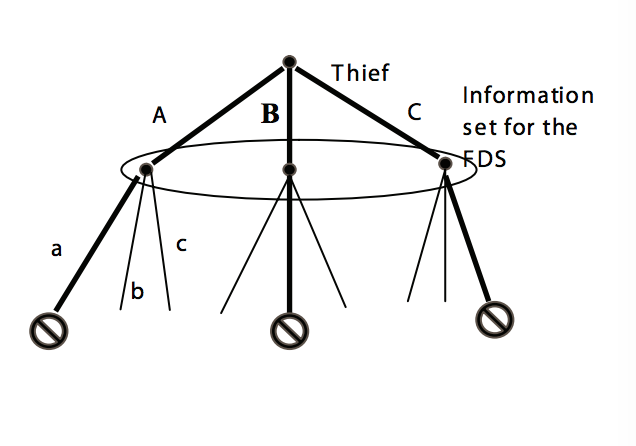
\includegraphics[scale=1]{gametheory.png}
  \caption{Rule Based Game Theoretic Approach: Search Structure}
  \label{fig:gametheory1}
\end{figure}

A transaction will go through two tiers before a final decision is made: a rule based tier and a game theory tier. The rule based tier calculates a suspicion score for each transaction; if the transaction fails the rule system, it is then sent through the second tier. In the second tier, a heuristic is calculated by going through the feature space. The authors model the problem based on parameters about the type of fraudster it is, the strategy space for both parties and the action space for both parties. The structure of how the heuristic is calculated is similar to a decision tree, as shown in Figure~\ref{fig:gametheory1}. The benefit of using this system is that if the system thinks that the fraudster is learning its strategy, it can change strategies, or can strengthen its beliefs if it thinks its learning the type of fraudster.    


% Game Theory 2 paper ADD TO MENDELEY & Bibtex file
%google  Dempster-Shafer equation latex
%\cite{Panigrahi}

Panigrahi et al similarly combine game theory with a rule based filter to create a fraud detection system. This system varies from Vasta et al's because it has 4 distinct phases. The system begins with a rule based filter, similar to those perviously described. Rules include an address check and outlier detection, where the system checks how much a transaction varies from a user profile as well as general rules. From this rule based system, transactions are put into three categories: fraud, non-fraud, and suspicious. 

To combine these rules, Panigrahi et al use Dempster-Shafer theory, followed by a transaction history database, and a Bayesian learner. The Dempster-Shafer theory assigns a fraud probability to an event based on the classification the transaction has from the rule based system. For example, if a transaction is classified as non-fraud in the address portion, it will have 0 added to its overall fraud probability prediction. Those results are then fed to a transaction history database, which compares the current transaction with the user's past transactions as well as a generic database of fraud. 

Information about how much the transaction is deviating from normal behavior in 4 mutually exclusive cases is then sent to the Bayesian learner. The Bayesian learner then calculates a suspicion score, which is combined with the earlier suspicion score using Dempster-Shafer again. Based on a threshold, a transaction is then classified as fraud or non-fraud. A visualization of this system can be seen in Figure~\ref{fig:gametheory2}. Through their experiements, Panigrahi et al find that 0.3 and 0.7 are the most accurate lower and upper bounds, respectively, and that their system increased the true positive rate by about 15-20\%. 


%% add equation for Dempster Shafer

\begin{figure} \centering
  \includegraphics[width=\textwidth, scale=1]{GameTheory2.png}
  \caption{Architecture of Rule Based Filter, Dempster-Shafer Adder, Transaction History Database, and Bayesian Learner}
  \label{fig:gametheory2}
\end{figure}


\subsection{Auditing with Game Theory}
% ADD TO MENDELEY & Bibtex file

Game theory concepts can also be leveraged in the auditing context. Wilks and Zimbelman study the current financial auditing methods and offer suggestions for improving systems adding game theory. The authors describe that there are several levels of reasoning: zero order, first order, and higher order. Zero order logic occurs when a user is only considering conditions affecting themselves. First order is when a user considers some conditions, and higher order is when a user considers multiple levels of reasoning and layers of complexity. Since fraud and fraud detection are games highly reliant on opponent's moves, strategy can change drastically based on response from the other player. This is inherently difficult because either parties' next move is highly dependent on the other's move. 

Currently, the best practices of the auditing field require auditors to go through a checklist of ``red flags". While this is very effective for first order reasoning, it does not catch any fraudsters that are reacting to changes in the ``red flag" checklist. The authors point out that these checklists have been shown to be less sensitive than intuitive fraud risk models. This is in part because of the dilution effect, where an auditor is focusing on too many irrelevant cues instead of the relevant cues. 

Instead, the authors suggest decomposing the decision into multiple components, making a judgement on each of these components, and recombining to make a global decision. The three elements the authors contribute to fraud are known as the ``fraud triangle": incentive, opportunity, and attitude. The authors also suggest that having auditors meet with their clients and look for in person cues helps auditors learn cues and potentially fraudulent behaviors. Through this process, Wilks and Zimbelman find that accuracy improved in low risk fraud situations, but did not improve high risk situations. They also found that attitude cues are easily concealed, and that auditors often were anchored to their initial judgements, and were unlikely to change their minds given new information.

Through their experiments, the authors offer advice that can be applied to audits as well as credit card fraud detection. The two main components the authors suggest adding are unpredictability and strategic reasoning. Unpredictability can be achieved by changing the time line of the fraud detection or audit, as well as changing the way the system works from time to time. This unpredictability can help catch fraudsters that were not anticipating an audit, and therefore might not have hidden their work as well. The authors also suggest adding opportunities for auditors to learn strategic reasoning, and increase their intuition. 

While this is true of humans, it is also true of fraud detection systems, as models also need the opportunity to engage with new fraudulent behavior to learn new patterns. Through incorporating human intuition into computerized systems, fraud detection systems can continue to move towards taking all analysts out of the process of fraud detection. Without it, companies will continue to argue that humans have intuition machines do not, requiring overhead from manual transaction processing. 




\noindent

\pagebreak
\chapter{ Fraud in Context}
\label{sec:context}

Most computer science research is dedicated to finding the most accurate and most efficient methods of solving a problem. This is a great standard for research, but in many contexts, results from research may not be as applicable in the real applications. In an attempt to understand the differences between related works in fraud detection and companies detecting fraud in the present. Through these interviews, I gained more knowledge into real world fraud detection.

\section{ Interviews from Professionals}

To gather a sense of business level fraud detection methods, I interviewed four professionals in the industry. Two of the people I interviewed have directly dealt with credit card fraud in their line of work. The third person I interviewed has worked in the British government, then transitioned into insurance fraud detection, and has spent large amounts of time tracing insurance fraudsters. The last interviewee has a doctorate in engineering, but has worked in fraud detection for many different industries. As a caveat, I will not be referencing these participants by name or by organization. Through these interviews, I found that fraud is handled slightly differently depending on the principles and restrictions of a business.

To start, my first credit card fraud expert began by explaining the different forms of fraud that a company looks out for. There are two main types of transactions that credit card companies are concerned with: physical and non-physical. There are a plethora of ways to spend money online that do not result in physical purchases, and each type of purchase comes with its own set of information. The straight forward, rules-based method of detecting fraud comes from the billing address zipcode, CVV, and computer timezone. When purchasing online, the first step is to verify that a CVV does indeed match with the credit card number. After this, one can check that the timezone of the zipcode is close to the timezone the computer is in. While a business will get a negative response from the credit card company if the CVV or the zipcode does not line up with the saved information, the timezone on a computer is often faked leading to further deception. With physical goods being sent to an address, one way of detecting whether it is fraud is to check if the delivery address is a normal building, and not an abandoned warehouse. Location can also be verified in other contexts such as airline credit cards and banking apps. Airline cards for example can keep information about when you are going to fly places, and not cancel your credit card when you appear in a different country after only a few hours. Banking apps can pull out location information from an app request independent of a transaction to verify that the user is in the same place.

Fraudsters have found sly paths around many fraud detection systems. While it would be optimal to cut off all paths of fraud, credit card information is continually circulated and sold to fraudsters. However, these fraudsters don't know which cards are currently in use. One way fraudsters have found to solve this problem is through leveraging free trials. A fraudster can sign up on Spotify or Netflix for example for a free trial. If the card information is good enough to pass these slightly less stringent free trail gates, that means the card information is good to use in other situations. Once the card is used in real life, the owner of that card gets the charge. To make these fraudulent dealings look more realistic, fraudsters have started using computers from the area associated with the card and using that computer for a reverse geoIP, which can then be used to proxy the transaction. Through this process, these transactions look more legitimate because the locations seem plausible. 

While fraudsters have technical solutions to help hide themselves, there are methods of detecting this behavior. When a fraudster gets a list of credit cards, they usually use a bot to go through the list of cards and do the process mentioned above. These series of transactions normally take too little time for a human to have completed, and come from the same IP address. The interviewee's company analyzed these sort of bot transactions, looking for the same bot trying to do similar fraudulent transactions on multiple sites. 

Surprisingly, many companies choose to buy fraud detection software rather than working in house. Banks for example use Falcon software, which looks at the flow of transactions in order to pinpoint suspicious transactions. Banks are an interesting case because they have such a high volume of transactions that they can afford to do these type of velocity checks. On the merchant side of the world, most physical goods merchants don't use much fraud detection at all and rely on the chip and basic credit card security. This may be because in the past a merchant would not be responsible for a fraudulent transaction if they had a swipe of a credit card and a signatures. It is also a question of risk versus reward and what you are selling. If you are selling diamonds, you may be more concerned with fraudulent transactions than if you are selling Beanie Babies. There are many filters for online transaction fraud such as Retail Decisions as well as 41st Parameter. These filters check for many red flags, including if the same browser is buying again and again. Companies with longer term transactions have the flexibility to involve customer service members in the fraud detection process, as they have time to verify a transaction for a tangible good. For intangible goods such as Netflix, there is less flexibility as it is an instant decision. 

One last example the interviewee mentioned explains how fake physical credit cards are constructed. Once you know you have a valid card, you can magnetically create a card using a room key. While this key does not look real, you can go buy gas with it and if people aren?t paying attention go to the store. If you are more sophisticated, you can clone the card, which is much harder to do with the chip so strip will eventually go away so when you are using the card you?re much less likely to be fraud. An online fraud example involves selling iPhones. A fraudster gets a spam person to ship a real phone, take packages and mule for the fraudster and then Amazon or whatever vendor is out that cost. These plans work effectively only if not caught by local agencies or the Counterfeiting and Banking sector of the Secret Service. 

The second fraud export I spoke to is part of a broader fraud detection team at a company with multiple product lines. The specific team works to detect and handle fraud and abuse across all of the company. However, he in particular helps on the credit card fraud detection sector. Since this company is larger, it has the resources to create its own fraud detection systems, which are heavily biased towards applied machine learning techniques. While this is a modern company, according to the interviewee, they use older machine learning techniques and apply them to new problems. They are not necessarily looking to upgrade their systems when new research comes out. Instead, they look for ways to enhance their system based on the problems that come up. They focus on supervised and reinforced learning for their fraud detection.

Like some of the related work, the interviewee emphasizes how fraud and security are very different problems than others because the problem is always changing. A contrary example to fraud detection is training a model to detect cancer using MRIs and scans. Here, once the classifier is trained, it will be mostly accurate for its niche. With fraud detection, by setting a model, fraudsters will change their behavior accordingly. Therefore, one classifier will never suffice for long periods of time. Because of the heavy interactions with humans with poor intentions, it is best to combine the machine learning with game theory in order to both catch and block fraudsters. For example, there is a push and pull relationship when attempting to find fraudsters. While attempting to pursue a fraudster and cut off their fraud channel, there is a risk of losing that fraudster again. According to the interviewee, there is a lot less push and pull when using a specific model, rather than changing models frequently.

Though model choice can affect results, the interviewee argues that it is not the most important element to accuracy gains. There are large differences in the macro level techniques like convergence models, linear models and others, but there is not a particular model that is perfect. Since the problem is changing so quickly, it is best to find the model that is closest without trying to find the perfect solution. Instead, the dataset is much more important than the actual model. With changing fraudulent behavior, it is better to implement new parameters rather than change the model. 

However, there are draconian restraints on data a company can have as well as privacy concerns. For example, this company does not track users locations for use in fraud detection, and restrict other elements of the data before ever reaching the fraud detection team. The mantra here is to put the fraud detectors in a position where it would be impossible to do bad things to people in the future based on the data they have. The loophole here is that some of the restricted data can be used by running the models on device rather than at the company, meaning the fraud team or company as a whole never sees restricted elements of data. These restraints can make fraud detection difficult because the models have to learn user's behavior without seeing the data and gauge their ``health" in the system. Through these constraints, fraud detection becomes an even more difficult problem.

The next person I interviewed has had a large range of jobs, investigating, analyzing, managing, and developing intelligence in all incarnations of fraud and corruption. While he is focused in insurance fraud at the current moment, he has worked in welfare fraud, investment banking ``Rogue Trader" profiling, and terrorist funding to name a few. His team and his work in investigating terrorist funding has actually prevented a few bombing attacks on London, emphasizing again the importance of fraud detection. 

In the industries this person has worked in, he has become a proponent of fraud analytic systems in rule based systems with human input. In his experience rule based systems are less expensive and some what more effective than feature based systems. Feature based systems are expensive because of the work to continually increase and change the feature space. Rule based systems are easy to change and with a field investigator looking over the results is a highly effective an inexpensive solution. FICO for example has a rule based engine. For any of these systems, in Britain, there is a large repository of information about people which is incorporated with census data. This information can be leveraged by British companies for fraud detection. While insurance fraud is different than financial fraud because it is on the back end of an issue and financial fraud is trying to be stopped in the front end, they still have a lot of overlap of methods.

This insurance fraud expert referred to some of the work done by the last person I interviewed in the behavioral analytics space. The form of fraud detecting used behavioral analytics to try to spot fraud before the fraud even occurs. The system measures the likelihood of someone committing fraud at a high degree, and the system was able to reduce deductions in payouts for insurance claims by about 12\%. However, this sort of system is the ``Rolls Royce of fraud detection" as it is very expensive. In the insurance fraud expert's experience, organized crime will employ their best people to combat the fraud detection systems and threaten people on the inside to get their purpose. Therefore, it is quicker to get a rule based system up to speed in the short term, though feature based systems would most likely pay off in the long term.

In addition to the behavioral analytics, the last person I interviewed has also worked in banking, insurance, and online gambling fraud. Each of these fields are somewhat different because of the levels of security and data. Banking is probably the most traditional and secure sector. They are very slow and need to anonymize all data before taking it out of their premises. While all industries have certain levels of regulations, banking is particular strict with their security and users' privacy. However, because of the amount of transactions banks handle, they can provide researchers with much more data than insurance. Banks also have to have a reason for suspecting fraud for regulatory reasons, which can be difficult when using machine learning models. 

Insurance and gambling are slightly different than banking. One of the major issues with fraud detection in insurance is that sometimes there are no fraudulent transactions in a data set, and the actual amount of data is small. To get more data, insurance companies are attempting to get users to use their apps and extract more information from there. Gambling is different than either of these fields because it is the most open and have more relaxed laws than banks or insurance companies. Because of this, they are able to work much faster. Most techniques are transferable between these industries, but it is still important to have experienced people working on the problem, as the interviewee before also referenced. 


\section{ Research Versus Reality}

Through talking with these professionals, one point that was reemphasized was the cost of false positives over false negatives. This was the topic of discussion in many of the papers I read, and the professionals I talked to continued to stress the point. An interesting point to this is that companies generally accept some amount of fraud in their business, with about 1\% of transactions being an acceptable amount of fraud for a company. While 1\% is quite small, this is a large amount of money when you consider some companies may be having millions to billions of transactions go through their system every day. Because of this, it seems that using a cost equation based on cost of the size of a transaction versus the number of correct and incorrect transactions would be beneficial. This way, the system would learn to pick up on high valued fraud instead of many small transactions.

The experts I interviewed all incorporated more human insight into their detection system than much of the research would suggest. Based on the very accurate results most of the related work has achieved, it would seem that companies would be able to fully automize their fraud systems. However, human intuition has continually trumped automatic systems in accordance to the four interviewees. Human involvement seems to have three factors associated with it: intuition, cost, and regulations. The intuition a human can bring to a fraud detection system relates to game theory. Fraudsters and analysts are essentially playing a game where both parties are profit maximizing, and are in a cat and mouse situation. Using human logic about how a fraudster will act is something only expensive machine algorithms may be able to do. A human can set up a rule based system using knowledge from past fraudulent behavior and expectations of where weaknesses in the system might lie. A behavioral machine learning algorithm is more computationally expensive, meaning that companies may not want to invest the money into a complex system. 

Lastly, humans will most likely always have to be part of the process because of regulations. When a customer is refused for a loan or creating a new credit card, there must be a reason associated with that decision to ensure there is no bias in the institution. Unlike somewhat unpredictable machine learning algorithms, a fraud analyst can easily point to how a rule based system created a denial decision. Through these interviews, I have found the reverse of what I expected: companies are actually not keeping up with newly researched methods but are actually opting for less expensive steadfast systems that have been in place for years. 


\pagebreak
\chapter{Implementing a Fraud Detection System}
\label{sec:impl}


%%% TODO IN THIS CHAPTER: 
% check that sum statistics are correct
% fill out the results section and tables
% write discussion section

To understand further the complexity of creating a highly accurate fraud detection system, I implemented my own system based on the approaches discussed in Chapter~\ref{sec:background}. I constructed a series of machine learning models, and reported accuracy and F1 scores based on different proportions of fraud to non-fraud data. For all experimentation, I used open source tools built for Python. I will discuss the model and the experiment in depth in the sections below. The overall implementation is broken down into subsections under Experiment: Hypothesis, Data, Methods, Results, and Discussion. 

\section{Model} %% Add in any extra models that I add after 10/29

For this project, I will be implementing several different machine learning models. I will be following 2011 Perols and will be comparing the performance of several popular classification models. To start, I will be implementing logistic regression.

%% diagrams from https://tex.stackexchange.com/questions/132444/diagram-of-an-artificial-neural-network


\begin{figure}

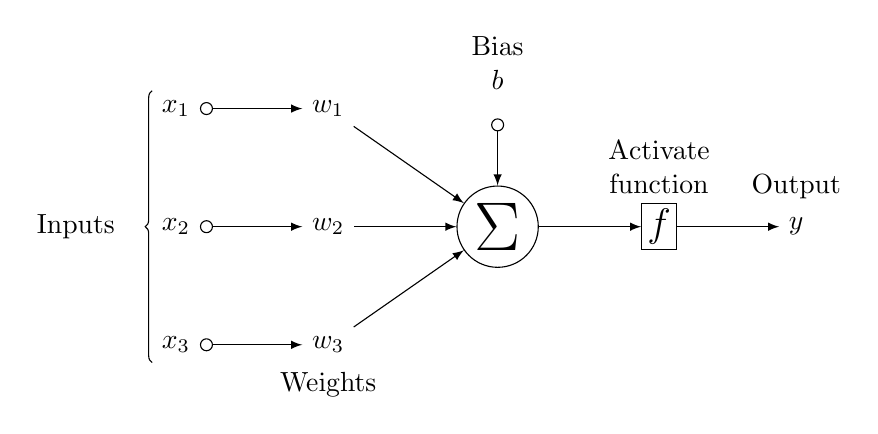
\begin{tikzpicture}[
init/.style={
  draw,
  circle,
  inner sep=2pt,
  font=\Huge,
  join = by -latex
},
squa/.style={
  draw,
  inner sep=2pt,
  font=\Large,
  join = by -latex
},
start chain=2,node distance=13mm
]
\node[on chain=2] 
  (x2) {$x_2$};
\node[on chain=2,join=by o-latex] 
  {$w_2$};
\node[on chain=2,init] (sigma) 
  {$\displaystyle\Sigma$};
  \node[on chain=2,squa,label=above:{\parbox{2cm}{\centering Activate \\ function}}]   
  {$f$};
\node[on chain=2,label=above:Output,join=by -latex] 
  {$y$};
\begin{scope}[start chain=1]
\node[on chain=1] at (0,1.5cm) 
  (x1) {$x_1$};
\node[on chain=1,join=by o-latex] 
  (w1) {$w_1$};
\end{scope}
\begin{scope}[start chain=3]
\node[on chain=3] at (0,-1.5cm) 
  (x3) {$x_3$};
\node[on chain=3,label=below:Weights,join=by o-latex] 
  (w3) {$w_3$};
\end{scope}
\node[label=above:\parbox{2cm}{\centering Bias \\ $b$}] at (sigma|-w1) (b) {};

\draw[-latex] (w1) -- (sigma);
\draw[-latex] (w3) -- (sigma);
\draw[o-latex] (b) -- (sigma);

\draw[decorate,decoration={brace,mirror}] (x1.north west) -- node[left=10pt] {Inputs} (x3.south west);
\end{tikzpicture}
\caption{Logistic Regression}
\label{fig:lr}
\end{figure}

Linear regression is a way to estimate the best fit line through a set of points. The best fit line is the line that minimizes the squared error of each point in relation to the estimation on the line. This algorithm is used to create a relationship between points, and to analyze the relationship between points \cite{Swaminathan}. As more freatures are added to the estimation, the regression increases in complexity. Logistic regression is different from linear regression only in the equation used to estimate the relationship between the points. Logistic regression is a wave shape that has limits at 0 and 1. Along the wave represents probabilities of an event given another feature. For example, logistic regression can model studying for a test: based on the number of hours you study, you can calculate the likelihood of passing that test. It is a particularly good method for classifying a binary variable because it calculates the probability that something is equal to 1 based on the given inputs.



\begin{figure}
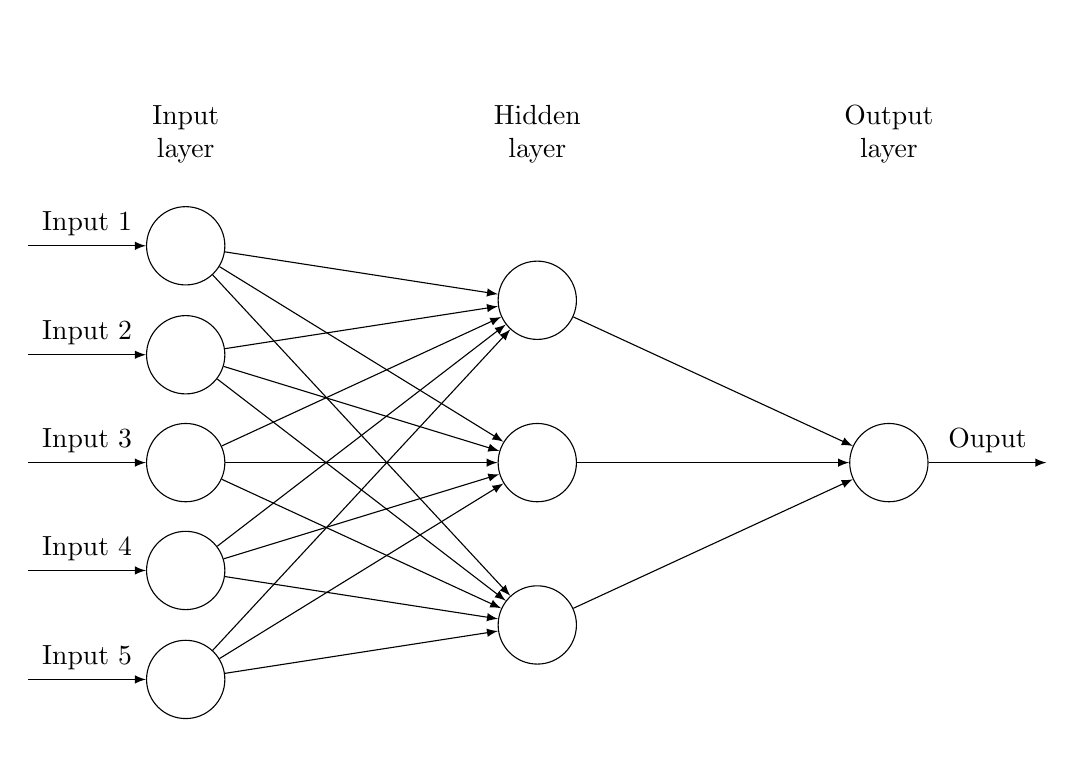
\begin{tikzpicture}[
plain/.style={
  draw=none,
  fill=none,
  },
net/.style={
  matrix of nodes,
  nodes={
    draw,
    circle,
    inner sep=10pt
    },
  nodes in empty cells,
  column sep=2cm,
  row sep=-9pt
  },
>=latex
]
\matrix[net] (mat)
{
|[plain]| \parbox{1.3cm}{\centering Input\\layer} & |[plain]| \parbox{1.3cm}{\centering Hidden\\layer} & |[plain]| \parbox{1.3cm}{\centering Output\\layer} \\
& |[plain]| \\
|[plain]| & \\
& |[plain]| \\
  |[plain]| & |[plain]| \\
& & \\
  |[plain]| & |[plain]| \\
& |[plain]| \\
  |[plain]| & \\
& |[plain]| \\    };
\foreach \ai [count=\mi ]in {2,4,...,10}
  \draw[<-] (mat-\ai-1) -- node[above] {Input \mi} +(-2cm,0);
\foreach \ai in {2,4,...,10}
{\foreach \aii in {3,6,9}
  \draw[->] (mat-\ai-1) -- (mat-\aii-2);
}
\foreach \ai in {3,6,9}
  \draw[->] (mat-\ai-2) -- (mat-6-3);
\draw[->] (mat-6-3) -- node[above] {Ouput} +(2cm,0);
\end{tikzpicture}
\caption{Neural Network}
\label{fig:nn}
\end{figure}

Artificial neural networks leverage logistic regression to build systems that can solve more complex problems. Neural networks are created by combining multiple nodes in different layers to create a network \cite{Suryansh}. Here, nodes represent logistic regression, as they take in inputs, estimate based on those inputs, and output an answer. The general structure of a neural network is to have an input layer, one or more hidden layers which can be of any size, and an output layer. Information is propagated forward through the network, and then back propagated again to adjust the parameter estimates of each node. Through this forward and backward process, the system eventually reaches a minimum, where the difference between the predictions and the real values is minimized. After the training period, the network has now been trained, and can calculate an output for any new input. This system is extremely powerful, and can be tuned significantly based on learning rate, hidden layer numbers, activation functions and other features of the network. 

Decision trees are somewhat similar to neural networks, but instead of traversing a network, decisions are made through branching at features. Each parent node represents a decision or feature and the children nodes represent the outcomes of said feature. Cost functions are used to find the most homogeneous branches, or branches with similar inputs. Decision trees can grow arbitrarily large, and sometimes require pruning to avoid a long prediction process. In addition, decision trees can be combined to create decision forests, further enlarging the architecture and complexity of the learning model \cite{Gupta}. When using a decision forest, a tree would act as a branch in a single tree, focusing on learning on feature. Like neural networks, there are also many parameters to tune, and architecture elements to adjust such as maximum depth and minimum number of training inputs.

A slightly different approach to this classification problem is using probability distributions such as a Gaussian distribution. The idea behind this classification is that anomaly data is almost always not the anomaly. Therefore, assume all the data you have is the majority class. If this data is approximately normally distributed, then you can calculate the probability of a new example being part of the majority class. Since anomalies are infrequent, they have low probabilities of being part of the majority class, and therefore are most likely anomalies. The last step of this approach is to choose a threshold for how likely an example must be to be classified as an anomaly. 

The last classification method I will be discussing is support vector machines or SVMs. SVMs classify data into categories by finding the most accurate boundary line to divide the data \cite{Brownlee}. This is particularly simple with a binary example like fraud detection. Here, we use kernels to calculate the plane or division that best splits the data with the lowest error rate. Like neural networks, to find the most accurate split between the data, we implement stochastic gradient descent to find the minimum cost points. Once this division is created, predictions are made based on the location of a point of interest in regard to the line dividing the data. 

\section{Experiments}

I will be experimenting with the models listed above to model the best classifying algorithm possible. The experiments will be two fold. I will be experimenting with the distribution of the data and with the parameters and hyper-parameters of the data. In Perols' paper, he finds the best results when looking at an equal split of fraudulent and non-fraudulent transactions \cite{Perols2011}. I would like to replicate his study by altering the proportion of fraud to non-fraud, and compare results. I will also be experimenting with the structure of the models themselves. As discussed above, each model has several many elements that can be tuned to find the best results. Neural networks in particular can take many forms, and require certain levels of trial and error to find the best results. Through these two axis, I will compare the performance of each model both to other models in this thesis and performance in Perols' paper. 


\subsection{Hypothesis}

Based on Perols' paper, I hypothesize that the best results will come with more equally distributed data. I think that neural networks will perform best because they are able to capture patterns in the data unseen by an analyst, and may perform better than the other models I have selected. However, given enough data and the correct tuning, all of the tested models should theoretically approach the same accuracy levels. 

\subsection{Data}


The data used from this project was obtained from Kaggle.com \cite{paysim}. I used the ``Synthetic Financial Datasets for Fraud Detection" which was generated by the PaySim mobile money simulator and is scaled down to a quarter of the original dataset \cite{paysim}. The dataset includes attributes about type of the transaction, amount, the customer that started the transaction, the initial balance of the sender, the balance after the transaction of the sender, whether its fraud, and other variables. The summary statistics are shown in Table~\ref{sec:sumstats}, and example of the information displayed in one transaction is displayed in Table~\ref{sec:example}.

\subsubsection{Limitations}

This project was limited by the dataset I had access to. In the real world, a transaction would include much more information that is not available with the fields of Paysim. Banks and credit card companies for example have the ability to see exactly where a transaction took place. As discussed in Chapter~\ref{sec:context}, banks and companies have strict policies they have to follow in regards to sharing user data. Therefore, there are no readily available datasets online. For reference, in the paper by Chan et al referenced above, their dataset had 30 fields per transaction \cite{Chan}. Some banks pull information from their own banking app on a user's phone and compare the location of the user's phone to the location of the past transaction. With credit card information, companies can detect fraud based on if transactions are occurring in two places very far away from each other. Since I do not have any sort of location information, I cannot leverage this type of rule based fraud detection. In addition, I do not have access to the name of the business a transaction is taking place at. By building out a user profile that includes frequent locations and businesses the user goes to, a detection system can detect if a person is shopping at a store that is out of the norm and calculate the likelihood that this is fraud. 


\begin{table}[htbp] \centering
\def\sym#1{\ifmmode^{#1}\else\(^{#1}\)\fi}
\caption{Summary Statistics\label{tab1}}
\label{sec:sumstats}
%\vspace{-18 pt}
\setlength{\tabcolsep}{15pt}

% %%%%%%%%%
\scalebox{1} {

\begin{tabular}{l@{\hskip 0.5in} c c c c}\addlinespace\hline\hline
\addlinespace
%\multicolumn{1}{c}{}&\multicolumn{3}{c}{2009 to 2015}\\
Transaction Measure&Mean&Min& Max\\
\hline

\addlinespace
\addlinespace													
\multicolumn{4}{l}{\textit{Legitimate Transaction}}\\													
Amount	 			     &	178,197    &	0.01	&	92,445,516 \\
%Old Balance Originator	     &	77.99	&	8.186	&	44.877	\\
%New Balance Originator	     &	17.54	&	7.09	&	3.66	\\
%Old Balance Recipient	     &	77.99	&	8.186	&	44.87 \\
%New Balance Recipient	     &	17.54	&	7.09	&	3.66	\\
Count = 6,354,407 				&		&		&		\\


\addlinespace													
\multicolumn{4}{l}{\textit{Fraudulent Transaction}}\\
Amount	 &	1,467,967	&	0	&	10,000,000 \\
Count = 8,213				&		&		&		\\

\addlinespace
\addlinespace
\multicolumn{4}{l}{\textit{Cash In}}\\
Amount	 &	168,920	&	0.04	&	1,915,267 \\
Count = 1,399,284				&		&		&		\\
\addlinespace
\addlinespace
\multicolumn{4}{l}{\textit{Cash Out}}\\
Amount	 &	176,273	&	0	&	10,000,000 \\
Count = 2,237,500				&		&		&		\\
\addlinespace
\addlinespace													
\multicolumn{4}{l}{\textit{Debit}}\\													
Amount	 &	5,483	&	0.55	&	569,077 \\
Count = 41,432				&	17.54	&		&		\\
\addlinespace
\addlinespace													
\multicolumn{4}{l}{\textit{Payment}}\\
Amount	 &	13,057	&	0.02	&	238,637 \\
Count = 2,151,495				&	&		&		\\
\addlinespace
\addlinespace													
\multicolumn{4}{l}{\textit{Transfer}}\\										
Amount	 &	910,647	&	2.60	&	   92,445,516 \\
Count = 532,909				&		&		&		\\

\hline\hline
\end{tabular}
}
\end{table} 

\begin{table}[htbp] \centering
\def\sym#1{\ifmmode^{#1}\else\(^{#1}\)\fi}
\caption{Example Transaction\label{tab1}}
\label{sec:example}
%\vspace{-18 pt}
\setlength{\tabcolsep}{15pt}

% %%%%%%%%%
\scalebox{1} {

\begin{tabular}{l@{\hskip 0.5in} c}\addlinespace\hline\hline
\addlinespace
%\multicolumn{1}{c}{}&\multicolumn{3}{c}{2009 to 2015}\\
Transaction Number & Category\\
\hline

\addlinespace
\addlinespace													

\multicolumn{2}{l}{\textit{Hour}}\\
Transaction 1 & 1 \\
\addlinespace
\multicolumn{2}{l}{\textit{Type}}\\
Transaction 1 & Payment \\
\addlinespace
\multicolumn{2}{l}{\textit{Amount}}\\
Transaction 1 &  \$9839.64\\
\addlinespace
\multicolumn{2}{l}{\textit{Name Origin}}\\
Transaction 1 & Alice \\
\addlinespace
\multicolumn{2}{l}{\textit{Old Balance Origin}}\\
Transaction 1 &  \$170,136.00 \\
\addlinespace
\multicolumn{2}{l}{\textit{New Balance Origin}}\\
Transaction 1 & \$160,296.36 \\
\addlinespace
\multicolumn{2}{l}{\textit{Name Destination}}\\
Transaction 1 & Bob \\
\addlinespace
\multicolumn{2}{l}{\textit{ Old Balance Destination}}\\
Transaction 1 &  \$0.00 \\
\addlinespace
\multicolumn{2}{l}{\textit{New Balance Destination}}\\
Transaction 1 & \$ 0.0 \\
\addlinespace
\multicolumn{2}{l}{\textit{Is Fraud}}\\
Transaction 1 & 0 \\

\hline\hline
\end{tabular}
}
\end{table} 



\subsection{Methods}

In order to implement my models, I will be leveraging the python package Sci-kit learn. Sci-kit learn has readily available implementations of major classifiers that I am interested in testing, as well as the infrastructure for predicting and analyzing the results of the models. I use the python package Pandas to read in and manipulate my data in a data-frame format. After reading in my data, I clean the data by selecting the fields I am interested in, and converting them to a usable format. For experiments where I am changing the distribution of fraud to non-fraud transactions, I extract the two transaction types from the total dataset. I then randomly sample a portion of the non-fraudulent transactions based on that experiment, and recombine that dataset with the entirety of the fraudulent dataset. This ensures that there is no selection bias in my results. 

Once my data is cleaned, I randomly split the data into training sets and test sets. I reserve about 15\% of my dataset for testing. I do this to ensure my model does not learn the patterns of the tests, so I can test the accuracy of the model when exposed to new information. With my data prepared, I then run my series of tests with different classifiers and different architectures. The results are shown below. 

As discussed in the experiment section, the majority of the methods employed are to test what alterations to my models creates large increases to accuracy and correct predictions. For each model, I used a subset of my data and altered the parameters and hyperparameters. Examples of this include changing the learning rate for the neural network model or choosing the max depth of the decision tree classifier. One of the main parameters I was interested in was the learner formula; which is the actual equation for which weights are calculated. This sort of guess and check method may seem somewhat misguided, but is one of the only ways to tune many machine learning algorithms. I focus on data manipulation as my computationally expensive tests. 

% maybe explain the different equations for learners?


Testing the neural network model is slightly more complicated, as you can have drastically different results based on the architecture. Neural networks are constructed of an input layer, output layer, and as many hidden layers in between as desired. Both the number of hidden layers as well as the number of nodes within each of the layers can be specified, growing or shrinking the model in complexity. In addition to the architecture, I will also be testing the epoch or max iterations parameter. An epoch is one forward propagation of data and one backward propagation. Each time data cycles through the network, the weights adjust and supposedly become more accurate. In addition to the other experiments, I will analyze the best amount of epochs for the fraud classification problem.

One of the elements of data manipulation I have tested is incorporating engineered features. The data I have is synthetic mobile payments as discussed in the data section. While this is a useful dataset for this project, it is somewhat limited in comparison to the information a credit card company would have on a normal brick and mortar transaction. The main limitation I attempt to expand upon is the lack of user profiling. There are over 6 million transactions in this dataset, with some of the same users repeating transactions. Each transaction includes information about which parties a transaction is between, the time as represented in hours and the amount. 

The other two elements of data manipulation I test are fraud to non-fraud data proportions as well as normalization. While Gaussian probability distributions are effective at anomaly detection, much of the related work in this field have leveraged standard classifiers as their most successful models. In order for these models to work correctly, they must see many examples of all classes of data in order to make accurate predictions. Since fraud detection is a binary problem, it is logical to assume a classifier will do best in an environment where it is learning with 50\% fraud and 50\% legitimate transactions. However, this is not always attainable in the real world, so I test with multiple data proportions, with fraud making up between 50\% of the transactions to less than 1\% using the unaltered dataset. In addition to this, I also test whether normalizing the data increases the accuracy of the classifiers. Normalizing stretches the data so that it is equally spread along a distribution, while maintaining the original proportions of data. The normalization equation can be found in equation ~\ref{eq:normal}. 


\begin{equation}
\label{eq:normal}
Normalized(transaction) = \frac{( transaction - min(transaction))}{  (max(transaction) - min(transaction))}
\end{equation}

Leveraging this information, I have created three additional fields: average transaction value for a user, time since last transaction, and whether a user has interacted with the destination user before. By calculating the average transaction amount, it may be more obvious when a fraudulent transaction that is either a lot higher or a lot lower than average occurs. Time since the last transaction is meant to see if a user has made many transactions in a short period of time. Although I do not have location data, it is still unlikely for a user to make a large amount of transactions in one hour. Lastly, I included an indicator for whether a user has interacted with the other user in the transaction before. It may be a sign of fraud if a user is interacting with a new user after many transactions with the same users. I decided on these three features because of human intuition, and what I think is possible between users. This is a large part of machine learning, as without the correct features, a system may not be able to classify effectively.

Arguably the most important element of a machine learning experiment is deciding how to quantify a successful algorithm. The most common method of measuring whether a model is improving or worsening is accuracy. As discussed above, this is helpful in more balanced class situations, but is a little biased when working on anomaly detection. Because of this, I include precision, recall and an F1 score of each model in addition to the accuracy. The equations for precision, recall and F1 are shown in equations ~\ref{eq:precision}, ~\ref{eq:recall}, and ~\ref{eq:F1}, respectively. 

\begin{equation}
\label{eq:precision}
    Precision = \frac{True Positives} {(True Positives + False Positives)}
\end{equation}

\begin{equation}
\label{eq:recall}
    Recall = \frac{True Positives}{ (True Positives + False Negatives)}
\end{equation}

\begin{equation}
\label{eq:F1}
    F1 = \frac{2 (Precision * Recall)} {(Precision + Recall)}
\end{equation}


As seen in the equations above, these measures are focused more so on the proportion of true positives to false positives. Precision describes a ratio of correctly identified fraud to all transactions identified as fraud. Recall is the proportion of correctly identified fraud to all identified as fraud. The F1 score is a measure incorporates both precision and recall, and is a helpful tool for combining these metrics. As discussed in ~\ref{sec:intro}, depending on the industry, false positives are often more expensive than false negatives. This is because it is sometimes less expensive to pay out for small levels of fraud rather than lose a potential client because of suspected fraud. Therefore, my analysis of results comes from both accuracy and the F1 score.



\subsection{Results}

The most successful models and their metrics are shown in the following tables. For trials with non-normalized data, refer to Table ~\ref{sec:non_norm_results}. Normalized results can be found in Table ~\ref{sec:norm_results}. 


\begin{table}[htbp]\centering
\def\sym#1{\ifmmode^{#1}\else\(^{#1}\)\fi}
\caption{Results: Non-normalized Data \label{tab1}}
\label{sec:non_norm_results}
%\vspace{-18 pt}
% %%%%%%%%%
\scalebox{1} {
\begin{tabular}{l@{\hskip 0.7in} c c c c} \addlinespace\hline\hline
\addlinespace
%\multicolumn{1}{c}{}&\multicolumn{4}{c}{2009 to 2015}\\
Method&Accuracy& Precision&Recall& F1 Score\\
\hline

\addlinespace
\multicolumn{5}{l}{\textit{Original data distribution}}\\
Logistic Regression	            &	0.9986	&	0.3735	&	0.493	&	0.425	\\
%Neural Network 	                &	0.998		&	0	&	0	&	0	\\
Decision Tree	            &	0.9997		&	0.8974	&	0.903	&	0.899	\\
SVM	        &	0.004		&	1	&	.0013	&	0.003	\\
Gaussian	        &	0		&	0	&	0	&	0	\\

\addlinespace
\multicolumn{5}{l}{\textit{50/50 data distribution}}\\ 
Logistic Regression	            &	0.905	&	0.899	&	0.911	&	0.905	\\
%Neural Network 	                &	0.998		&	0	&	0	&	0	\\
Decision Tree	            &	0.992		&	0.994	&	0.989	&	0.992	\\
SVM	        &	0.501		&	1	&	0.506	&	0.672	\\
Gaussian	        &	0		&	0	&	0	&	0	\\

\addlinespace
\multicolumn{5}{l}{\textit{66.6/33.3 data distribution}}\\
Logistic Regression	            &	0.910	&	0.854	&	0.885	&	0.869	\\
%Neural Network 	                &	0.998		&	0	&	0	&	0	\\
Decision Tree	            &	0.994		&	0.994	&	0.990	&	0.992	\\
SVM	        &	0.351		&	1	&	0.351	&	0.519	\\
Gaussian	        &	0		&	0	&	0	&	0	\\

\addlinespace
\multicolumn{5}{l}{\textit{75/25 data distribution}}\\
Logistic Regression	            &	0.931	&	0.839	&	0.880	&	0.860	\\
%Neural Network 	                &	0.998		&	0	&	0	&	0	\\
Decision Tree	            &	0.993		&	0.994	&	0.977	&	0.986	\\
SVM	        &	0.251		&	1	&	0.250	&	0.401	\\
Gaussian	        &	0		&	0	&	0	&	0	\\

\addlinespace
\multicolumn{5}{l}{\textit{80/20 data distribution}}\\
Logistic Regression	            &	0.938	&	0.820	&	0.880	&	0.850	\\
%Neural Network 	                &	0.998		&	0	&	0	&	0	\\
Decision Tree	            &	0.994		&	0.984	&	0.990	&	0.986	\\
SVM	        &	0.210		&	1	&	0.210	&	0.344	\\
Gaussian	        &	0		&	0	&	0	&	0	\\






\hline\hline
\end{tabular}
}
\end{table} 




\begin{table}[htbp]\centering
\def\sym#1{\ifmmode^{#1}\else\(^{#1}\)\fi}
\caption{Results: Normalized Data \label{tab1}}
\label{sec:norm_results}
%\vspace{-18 pt}
% %%%%%%%%%
\scalebox{1} {
\begin{tabular}{l@{\hskip 0.7in} c c c c} \addlinespace\hline\hline
\addlinespace
%\multicolumn{1}{c}{}&\multicolumn{4}{c}{2009 to 2015}\\
Method&Accuracy& Precision&Recall& F1 Score\\
\hline
\addlinespace
\addlinespace
\multicolumn{5}{l}{\textit{Original data distribution }}\\
Logistic Regression	            &	0.999	&	0	&	0	&	0	\\
%Neural Network 	                &	0.998		&	0	&	0	&	0	\\
Decision Tree	            &	0.999		&	0	&	0	&	0	\\
SVM	        &	0.999		&	0	&	0	&	0	\\
Gaussian	        &	0		&	0	&	0	&	0	\\

\addlinespace
\multicolumn{5}{l}{\textit{50/50 data distribution }}\\
Logistic Regression	            &	0.501	&	0	&	0	&	0	\\
%Neural Network 	                &	0.998		&	0	&	0	&	0	\\
Decision Tree	            &	0.499		&	1	&	0.499	&	0.666	\\
SVM	        &	0.538		&	0.498	&	0.541	&	0.519	\\
Gaussian	        &	0		&	0	&	0	&	0	\\

\addlinespace
\multicolumn{5}{l}{\textit{66.6/33.3 data distribution }}\\
Logistic Regression	            &	0.670	&	0	&	0	&	0	\\
%Neural Network 	                &	0.998		&	0	&	0	&	0	\\
Decision Tree	            &	0.330		&	1	&	0.330	&	0.497	\\
SVM	        &	0.330		&	1	&	0.330	&	0.497	\\
Gaussian	        &	0		&	0	&	0	&	0	\\


\addlinespace
\multicolumn{5}{l}{\textit{75/25}}\\
Logistic Regression	            &	0.750	&	0	&	0	&	0	\\
%Neural Network 	                &	0.998		&	0	&	0	&	0	\\
Decision Tree	            &	0.250		&	1	&	0.250	&	0.400	\\
SVM	        &	0.250		&	1	&	0.250	&	0.400	\\
Gaussian	        &	0		&	0	&	0	&	0	\\

\addlinespace
\multicolumn{5}{l}{\textit{80/20}}\\
Logistic Regression	            &	0.801	&	0	&	0	&	0	\\
%Neural Network 	                &	0.998		&	0	&	0	&	0	\\
Decision Tree	            &	0.801	&	0	&	0	&	0	\\
SVM	        &	0.801	&	0	&	0	&	0	\\
Gaussian	        &	0		&	0	&	0	&	0	\\



\hline\hline
\end{tabular}
}
\end{table} 




%- normalizing data actually got a slight increase in the accuracy by .01 across the board
%- also trying a Gaussian Probability model, which is what the ML coursera course recommends
%- setting up an experiment that runs through models of different architectures for different amounts of epochs and will also try with different Fraud/nonfraud distributions
%- may want to also play with alpha
%- will extend these experiments to my other test models



\subsection{Discussion}

This section will compare my hypothesis to the results, as well as my results to the model I'm basing it off of. I also plan on adding any notes I learn along the way of this implementation.


\pagebreak
\chapter{Further Applications}
\label{sec:future}


\section{Anomoly Detection}

\subsection{Cell Phone Fraud}

\subsection{Biometric Fraud}

\subsection{Bioinformatics}

\pagebreak
\chapter{Conclusions}
\label{sec:conclusion}


%\appendix
%\chapter{Chapter 1 of appendix}
%Appendix chapter 1 text goes here

\bibliography{thesis}

\end{document}
